\documentclass[10 pt]{article}
\usepackage[a4paper, total={7in, 9.5in}]{geometry}
\usepackage[spanish]{babel}
\usepackage{csquotes}
\usepackage{graphicx} 
\usepackage{caption}
\usepackage{hyperref}
\usepackage{graphicx}
\usepackage{float}
\usepackage{url}
\usepackage{color}
\usepackage{siunitx}
\usepackage{hhline}
\usepackage{multirow}
\usepackage[round]{natbib}
\bibliographystyle{plainnat}
\usepackage{todonotes}
\linespread{1.5}

\begin{document}

\begin{titlepage}

    \begin{center}
    \vspace*{-0.5in}
    \begin{figure}[htb]
    \begin{center}
    
\includegraphics[scale=.3]{images/uba2.jpg}
    \end{center}
    \end{figure}
    
    \begin{large}
    Maestría en Explotación de Datos y Descubrimiento del Conocimiento\\
    \vspace*{0.15in}
    Universidad de Buenos Aires \\
    
    \vspace*{0.6in}
    \end{large}
    
    \begin{large}
    TÍTULO DEL TRABAJO\\
    
    
    \end{large}
    \vspace*{0.2in}
    \vspace*{0.3in}
    
    
    \vspace*{0.3in}
    \rule{80mm}{0.1mm}\\
    \vspace*{0.1in}
    \begin{large}
    Victoria Colombo
    
    \vspace*{0.3in}
    
    \vspace*{0.1in}fecha
    \end{large}
    \end{center}
    
    \end{titlepage}

\newpage

\begin{abstract}

\end{abstract}
\newpage
\section*{Introducción}\label{intro}


La violencia sexual comprende una multiplicidad de conductas o intentos de conductas, que van desde actos hasta comentarios sexuales, dirigidos contra la sexualidad de otra persona de manera coercitiva. El trabajo con datos sobre violencia sexual presenta complicaciones porque los datos suelen ser escasos o presentar gran cantidad de faltantes \citetext{\citealp[p.~150]{ferris2002world}}. Uno de los motivos es que las víctimas o su entorno a menudo se rehúsan a denunciar o participar en encuestas sobre este tipo de agresiones, o proveen información incompleta. Esto puede deberse a la vergüenza y el estigma social frecuentemente asociado no solo con la violencia sexual sino con la sexualidad en general, pero también a la falta de acceso a la justicia, al temor a las represalias por parte de los agresores, o el temor a que la denuncia no sea creída \citep*{murphy2022unfounded}. Otros posibles motivos para la escasez y/o mala calidad de los datos pueden ser la falta de vías adecuadas para recabar esta información, o la negligencia o desconocimiento de procedimientos adecuados por parte de oficiales de policía encargados de recibir denuncias. A pesar de las dificultades en la recolección de datos, diversos estudios a nivel mundial logran identificar patrones frecuentes en la violencia sexual. Para este trabajo, resultan relevantes dos de ellos: la mayoría de las víctimas son mujeres, mientras que los perpetradores suelen ser hombres \citetext{\citealp[p.~149]{ferris2002world}; \citealp[p.~15]{contreras2016violencia}}; y en la mayoría de los casos, los agresores son personas conocidas por las víctimas, como parejas, exparejas u otros conocidos \citetext{\citealp[p.~9]{garcia2005multi},\citealp[p.~22]{unicef2018analisis}, \citealp[p.~151]{ferris2002world}}.
 
La clasificación de las identidades de género de víctimas y perpetradores es compleja. Por un lado, muchos estudios clasifican a las personas únicamente como hombres o mujeres, omitiendo las identidades de género disidentes.\footnote{Entre los estudios e informes consultados para este trabajo, solamente el \textit{Relevamiento de fuentes secundarias de datos sobre violencia sexual} de la \citet{ufem_relevamiento} menciona identidades de género cuando especifica que la violencia sexual “afecta particularmente a las mujeres cis y personas LGBTI+” (p.7).}. Por otro lado, aunque se reportan pocos casos de violencia sexual contra hombres cisgénero, es probable que estén subrepresentados debido a los prejuicios y estigmas sociales sobre la masculinidad que dificultan las denuncias y el acceso a la justicia para estas víctimas \citep*[p.~149]{ferris2002world}. Analizar esas complejidades excede a este trabajo de especialización. En mi análisis las categorías de género de víctimas, victimarios y llamantes se limitan a las registradas en el \textit{dataset}: hombre, mujer, y transgénero, sin especificar si es un hombre o una mujer transgénero. Reconozco esto como una limitación no solo de mi trabajo sino también de los datos disponibles.  

La  recopilación, sistematización, y análisis de datos sobre violencia sexual por parte de los Estados es crucial para planificar y llevar adelante políticas efectivas de prevención, asistencia, y erradicación de la violencia sexual. En Argentina, si bien no hay un sistema estatal único y centralizado de este tipo de información, existen entidades judiciales y programas estatales que, además de ofrecer auxilio, asistencia y/o acceso a la justicia, recaban datos sobre violencia sexual, y mantienen un registro público de ellos. Unos de esos programas es Las Víctimas contra las Violencias. 

Desde el año 2016, en el marco del programa Las Víctimas contra las Violencias, dependiente del Ministerio de Justicia de la Nación, la línea 137 funciona las 24 horas del día para solicitar asistencia en casos de violencia sexual o familiar\footnote{Además, desde 2020 cuenta también con el canal de \textit{Whatsapp} (54911) 3133-1000.}. El programa cuenta con equipos de intervención de abogadas, psicólogas, y trabajadoras sociales. Al recibir una llamada solicitando asistencia se coordina el envío de equipos móviles para proveer a la víctima, en base a las necesidades del caso, de contención emocional, acompañamiento a un hospital y/o a radicar una denuncia, y/o a un lugar seguro donde pueda alojarse \citep*{linea_137}.\todo{rever cómo sigue el programa ahora}

Los registros de las llamadas a la línea 137 se encuentran digitalizados desde 2017 y están disponibles en el \href{http://datos.jus.gob.ar/}{Portal de Datos Abiertos de la Justicia Argentina}. Allí se encuentran publicados cuatro tipos de \textit{datasets} por año: llamados e intervenciones domiciliarias por situaciones de violencia familiar, y llamados e intervenciones domiciliarias por situaciones de violencia sexual.
Los registros no están exentos de los problemas frecuentes antes mencionados en los datos sobre violencia sexual, ya que presentan información faltante de dos maneras: celdas vacías en el caso de las variables numéricas de edad, y respuestas NS/NC (no sabe-no contesta) en lugar de SI o NO en el resto de las variables categóricas. Teniendo en cuenta la clasificación de datos faltantes que se origina en \citet{rubin1976inference}, los datos faltantes en el \textit{dataset} de llamados son posiblemente del tipo \textit{missing at random} (MAR) y \textit{missing not at random/ non-ignorable missing data} (MNAR). Es decir, o bien los datos faltan por motivos que tienen que ver con otras variables (MAR), o bien el valor de los datos que faltan está relacionado con el motivo mismo por el que faltan (MNAR).

En este trabajo analizo llamados para reportar violencia sexual a la línea 137 entre 2017 y 2021, e intento predecir valores faltantes de la variable “víctima convive con el agresor”. 



\section*{Datos}\label{datos}

Para este trabajo descargué del \href{http://datos.jus.gob.ar/}{Portal de Datos Abiertos} mencionado arriba 5 \textit{datasets} en formato \textit{csv} de llamados a la línea 137 para solicitar asistencia por violencia sexual. Los archivos pertenecen, a razón de uno de por año, al período entre enero de 2017 y julio de 2021. 

Como primer paso, unifiqué los 5 archivos en un solo \textit{dataset}. Para eso fue necesario realizar una primera limpieza destinada a dejar consistentes los distintos archivos en términos de cantidad y nombre de columnas\footnote{La limpieza, normalización, y preprocesamiento del \textit{dataset} y la aplicación de los métodos exploratorios y predictivos fueron realizados en Python}:

\begin{itemize}
    \item Eliminé la variable \textit{caso\_id}, que solo existe a partir de 2020.
    \item Cambié el nombre de la variable \textit{llamado\_provincia\_indec\_id} en los \textit{datasets} de 2017, 2018, y 2019 a su equivalente en 2020 y 2021: \textit{llamado\_provincia\_id}.
\end{itemize}


El \textit{dataset} final unificado consta de 19143 observaciones y 54 variables, en su mayoría categóricas, que aportan información sobre la víctima, la persona que llama para reportar el hecho, el contexto del hecho y el tipo de violencia sufrida. En el cuadro \ref{tablavar} se puede ver un detalle de las variables y su tipo.

\begin{table}[H]
    \centering
    \caption{Resumen de las variables.}
    \label{tablavar}
    \begin{tabular}{|l|l|l|} 
    \hline
    \textbf{Descriptor} & \textbf{Tipo variable} & \textbf{Variable(s)}         
    \\ 
    \hline
    \multirow{2}{*}{Víctima} & Cuantitativa & victima\_edad 
    \\ 
    \cline{2-3}
     & Cualitativa & \begin{tabular}[c]{@{}l@{}}victima\_genero, victima\_nacionalidad, victima\_discapacidad, \\ victima\_vinculo\_agresor, victima\_convive\_agresor, victima\_a\_resguardo\end{tabular}          
     \\ 
    \hline
    \multirow{2}{*}{Llamante} & Cuantitativa         & {llamante\_edad}             
    \\ 
    \cline{2-3}
     & Cualitativa& llamante\_genero, llamante\_vinculo                  
     \\ 
    \hline
    \multirow{2}{*}{Llamado}& Ordinal & llamado\_fecha\_hora                                            
    \\ 
    \cline{2-3} & Cualitativa & \begin{tabular}[c]{@{}l@{}} caso\_id, llamado\_provincia llamado\_provincia\_id, \\ caso\_judicializado, hecho\_lugar\end{tabular}                                
    \\ 
    \hline
    Violencia sexual                 & Cualitativa  &  \begin{tabular}[c]{@{}l@{}} vs\_violacion\_via\_vaginal, vs\_violacion\_via\_anal, vs\_violacion\_via\_oral, \\ vs\_tentativa\_violacion, vs\_tocamiento\_sexual, vs\_intento\_tocamiento, \\ vs\_intento\_violacion\_tercera\_persona, vs\_grooming, vs\_exhibicionismo, \\ vs\_amenazas\_verbales\_contenido\_sexual, vs\_explotacion\_sexual,\\ vs\_explotacion\_sexual\_comercial, vs\_explotacion\_sexual\_viajes\_turismo, \\ vs\_sospecha\_trata\_personas\_fines\_sexuales, \\ vs\_existencia\_facilitador\_corrupcion\_nnya, \\ vs\_obligacion\_sacarse\_fotos\_pornograficas, vs\_eyaculacion\_partes\_cuerpo, \\ vs\_acoso\_sexual, vs\_iniciacion\_sexual\_forzada\_inducida, \\ vs\_otra\_forma\_violencia\_sexual, vs\_no\_sabe\_no\_contesta \end{tabular} 
    \\ 
    \hline
    Otras violencias & Cualitativa & \begin{tabular}[c]{@{}l@{}} ofv\_sentimiento\_amenaza, ofv\_amenazas\_explicitas, ofv\_violencia\_fisica, \\ ofv\_intento\_ahorcar, ofv\_intento\_quemar,  ofv\_intento\_ahogar, \\ ofv\_amenaza\_muerte, ofv\_uso\_sustancias\_psicoactivas, \\ ofv\_intento\_privacion\_libertad, ofv\_privacion\_libertad, \\ ofv\_uso\_arma\_blanca, ofv\_uso\_arma\_fuego, ofv\_enganio\_seduccion,\\ ofv\_intento\_matar, ofv\_uso\_animal\_victimizar, ofv\_grooming, \\ ofv\_otra\_forma\_violencia, ofv\_no\_sabe\_no\_contesta\end{tabular} 
    \\ 
    \hline
    \end{tabular}
\end{table}


\subsection*{Limpieza y exploración de los datos}
El siguiente paso fue limpiar los datos con errores de carga como ser de errores de tipeo, valores cargados con sinónimos o abreviaturas, o errores ortográficos:
\begin{itemize}
    \item Unifiqué en la variable \textit{victima\_vinculo\_agresor} el valor “Ex pareja de la víctima” que aparecía también como “Ex pareja”, “Ex-pareja de la víctima” y “Expareja de la víctima”, otro tanto hice con “Pareja de la vícitma” que presentaba variaciones similares.
    \item Unifiqué para todas las variables pertinentes los valores SI, NO, y NS/NC dejándolos en mayúscula, ya que aparecían en distintos formatos: minúscula, mayúscula inicial, etc.
    \item Sustituí todos los valores “Sin datos” por NS/NC por considerarlos equivalentes.
    \item Quité espacios de comienzo y final de \textit{strings} para solucionar problemas del tipo “Madre” =/= “  Madre” 
    \item Convertí en la variable llamante\_vinculo el valor “Vecino” a “Vecina/o” ya que  no necesariamente se refiere unívocamente a personas de género masculino.
    \item Unifiqué en llamado\_provincia “Ciudad Autónoma de Buenos Aires” y “CABA” optando por “CABA”. 
    \item Corregí en llamado\_provincia las instancias de “Santa Fé” a “Santa Fe”.
\end{itemize}
 

Las variables \textit{victima\_edad} y \textit{llamante\_edad} presentaban \textit{outliers}, como se aprecia en el \textit{boxplot} de la figura \ref{box_edades_log}, en el que los datos están escalados logarítmicamente para mejor legibilidad del gráfico. Dada la naturaleza de ambas variables, evalué los \textit{outliers} utilizando el sentido común y conocimiento de dominio antes que fórmulas clásicas como las cotas superior e inferior basadas en el IQR. De esta manera, los valores demasiado altos para ser la edad de una persona o demasiado bajos para ser la edad de una persona que llama por teléfono, los consideré errores de carga o bien números aleatorios ingresados para no dejar el campo vacío, y por lo tanto eliminé dejando las celdas vacías como datos faltantes\footnote{En el \nameref{anex} se puede consultar el cuadro \nameref{tabla_out}, con los valores que tomaban los \textit{outliers} eliminados en cada variable de edad, y comprobar que la mayoría eran 999 en ambas variables, muy probablemente un valor por defecto ingresado para no dejar el campo vacío.}. En total, removí 195 valores en \textit{llamante\_edad}, y 101 valores en \textit{victima\_edad}. 

\begin{figure}[H]
    \begin{center}
    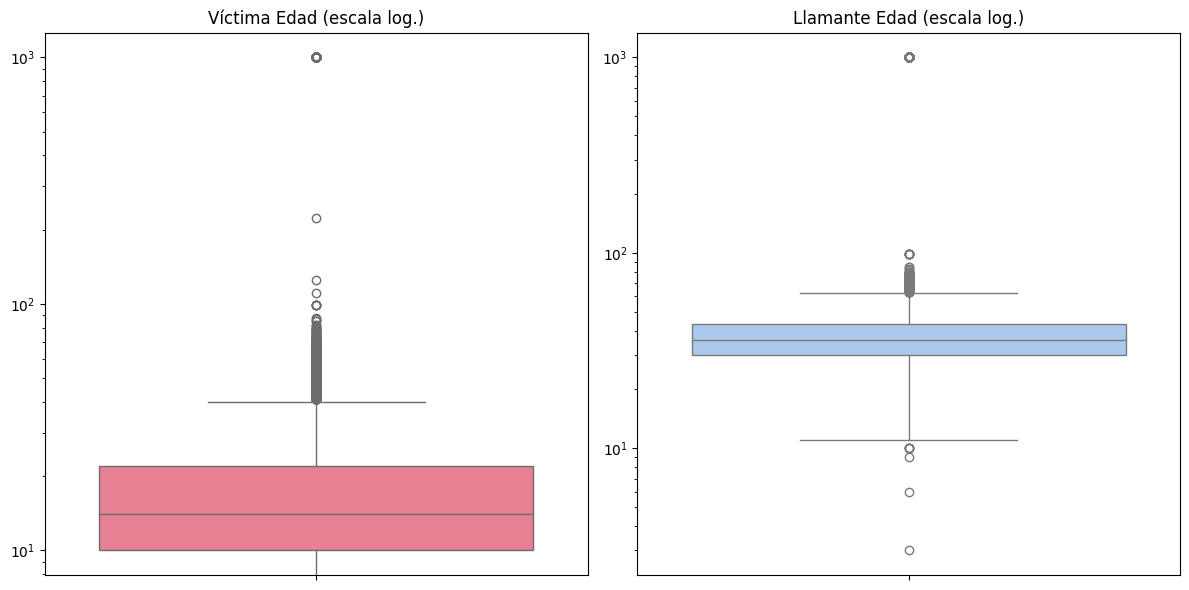
\includegraphics[scale=.5]{images/latex_boxplot_edades_outliers.png}
    \caption{Distribución las variables de edad en escala logarítmica.}
    \label{box_edades_log}
    \end{center}
    \end{figure}


Una vez removidos estos valores, tomé las medidas descriptivas de las variables de edad que se observan en el cuadro \ref{tabla_descr_ed}. Se puede ver que la mayoría de las víctimas no supera los 21 años, con una media de 17 y una moda de 14. Las personas que llaman para reportar los casos, en cambio, son en su mayoría adultos, con una media de 36 años, y una moda de 40. Esto refuerza lo mencionado en la introducción de hallazgos de otros estudios de que las personas más jóvenes y sobre todo los adolescentes e infantes son los grupos más en riesgo de ser víctimas de violencia sexual. 



    \begin{table}[H]
        \centering
    \caption{Medidas descriptivas de las variables de edad.}
    \label{tabla_descr_ed}
        \begin{tabular}{lcc}
        \hline
        \textbf{Descriptor} & \textbf{Edad de quien llama} & \textbf{Edad de la víctima} \\ \hline
        Media               & 36.25                        & 17.17                       \\
        Moda                & 40                           & 14                          \\
        Desvío Est.     & 11.41                        & 11.91                       \\
        Min.                & 3                            & 0                           \\
        25\%                & 29                           & 10                          \\
        50\%                & 35                           & 14                          \\
        75\%                & 42                           & 21                          \\
        Max                 & 99                           & 99                          \\ \hline
        \end{tabular}
        \end{table}


Según la distribución de la variable \textit{llamado\_provincia}, el 37\% de los llamados se realizaron en CABA; el \%36 en el resto de la provincia de Buenos Aires; del 9\% no se cuentan con datos; y el restante 18\% se reparte entre las restantes provincias del país, siendo de ese grupo Córdoba y Santa Fé las que más llamados tienen, con un 3\% cada una. \textit{hecho\_lugar}

Observé según la distribución de la variable \textit{victima\_nacionalidad}, que el 80\% de las víctimas son argentinas; del 15\% no se cuenta con datos sobre su nacionalidad; y el restante 5\% se divide entre las nacionalidades boliviana, paraguaya, peruana, brasileña, uruguaya, y chilena, y la categoría “otra”. Según la distribución de la variable \textit{victima\_genero}, \textit{victima\_discapidad}, \textit{victima\_vinculo\_agresor}, 

 
Además, construí la variable \textit{agresor\_conocido\_desconocido} para explorar la dicotomía extraños-conocidos en relación con las víctimas y los agresores

En cuanto a la variable de interés \textit{victima\_convive\_agresor}, 


Construí también las variables estación del año, fin de semana y momento del día para explorar frecuencia de los llamados. Exploré la variable provincia para ver la cantidad de llamados. 



Para ver interacciones entre la variable de interés \textit{victima\_convive\_agresor} y variables podrían estar relacionadas o aportar información que determine si el valor de la primera es más probablemente SI o NO,  realicé gráficos que exploran la relación entre \textit{victima\_convive\_agresor}, \textit{victima\_edad}, \textit{llamante\_edad}, \textit{llamante\_vinculo}, \textit{hecho\_lugar}, \textit{momento\_dia} (HACER UNO EDAD MENOR MOMENTO D´IA CONVIVE )



GRAFICOS P ESAS

Las variables de vs y ofv toman los valores SI NO.

En general en todas las variables de violencia hay muchos más NO que sí.

\subsection*{Datos faltantes}\label{faltantes}

datos faltantes en forma de NS/NC y en forma de datos vacíos. Dónde están y cuántos son. Cuántos en la variable de interés victima convive agresor. esto está en la notebook por qué faltan mis datos
Cuantos datos faltantes en edad de la víctima y edad del llamante esto está en la notebook por qué faltan mis datos

posible relación de datos faltantes de edad con quien llama tanto en edad de la victima como en edad de quien llama
relación entre los faltante de edad y NSNC en convive

relaci;on entre NSNC de convive y quien llama (instituciones) esto está en la notebook de por qué faltan mis datos y en las notas que tomé


\section*{Metodología}\label{met}

El objetivo es imputar los NS/NC de convive como si o no. 

Intento ver si usando un método de ordenamiento para visualizar el dataset en dimensiones reducidas me da una
idea de agrupamientos con repsecto a las tres categorías de convive. Elijo NMDS porque me permite trabajar con
variables de distinto tipo sin transformaciones.
 Luego, para intentar predecir los NSNC como si o no usé SVM. 

A modo de un segundo preprocesamiento para poder llevar a cabo estas tareas, decidí reducir las dimensiones del dataset a mano primero agrupando variables y reduciendo la cantidad de categorías en algunas otras variables. lA REDUCCI´OND E CARDINALIDAD DE algunas variables es especialemnte útil para la aplicación de SVM ya que esta conlleva encodear las features y para uno de los encoders elegidos, one-hot, la alta cardinalidad de features puede resultar problemática.


Habiendp hecho los gráficos de más arriba para explorar posibles interacciones entre dos o tres variables, me pareció valioso explorar más dimensiones y plasmarlo en dos dimensiones. Para eso apliqué NMDS

Reducción manual de dimensiones
Algunas resultan muy poco informativas como vs explotacion sexual viajes turismo (0,02) y ofv intento matar (0,01) resultan muy poco informativas (ocurrencia de 0,02 y 0,01). 

Despues medí correlación para ver si podía sacar más variables pero al final no saqué ninguna. Explicar cómo queda el dataset final

Después apliqué encoders para hacer SVM e hice SVM con la librería tal y con una búsqueda de hiperparámetros. Además experimenté con diferentes versiones del dataset cambiando la variable edad numérica por su contraparte categórica. Esto me peritió medir el posible impacto de los datos faltantes de edad. Cuando la edad era numérica, debía dejar afuera los datos faltantes ya que SVM no puede utilizarlos. Para poder utilizar todos los datos completos de edad, pasé la edad a categorica  utilizando las categorías tal tal y tal y dejado como NSNC los datos faltantes. Teniendo en cuenta estas variaciones en el tratamiento de la variable edad, los experimentos que realicé con SVM fueron: 
tal tal tal

cada uno probando los siguientes hiperparámentros

VER DE ARMAR UNA TABLA QUE RESUMA ESTAS VARIANTES 


\section*{Resultados}\label{resultados}
NMDS vemos que no hay en ninguna de las veriones del dtaset que usé una separación clara entre las categorías de interés.

VER DE RE ARMAR NMDS y que separe solo SI de NO y luego un tercero que haga SI NO NSNC

Todos dieron bien y luego el mejor modelo lo apliqué a 

\section*{Discusión y conclusiones}\label{conc}
cruzamiento de datos ovd líneas de asistencia, observatorio de género.
acceso y análisis de datos extensivo a provincias, no solo benos aitres


VER DE EN SVM RESULTANTE FINAL A LOS QUE LES PUSO S´I CU´AL ES LA EDAD DE V´ICTIMA Y A LOS QUE LES PUSO NO, CU´AL ES

en \textit{La guerra contra las mujeres}, \citeyearpar{segato2016guerra}, Rita Segato habla de la violencia sexual como algo siempre dirigido hacia cuerpos femeninos y \textit{feminizados} (resaltado propio). Con esto último quiere decir cuerpos percibidos o construidos por los abusadores como femeninos con respecto a posiciones de poder: menores, débiles, racializados, pertenecientes a disidencias sexuales. Esto se condice con datos sobre la mayor incidencia de la violencia sexual contra identidades masculinas durante la niñez y la adolescencia, es decir, en períodos en que los cuerpos y los sujetos son más vulnerables, y por lo tanto, también percibidos como feminizados \citep*{contreras2016violencia,ufem_relevamiento,ferris2002world}.

Si las denuncias de violencia sexual contra disidencias de género representan una minoría en los datos, ¿quiere decir esto que esas personas sufren menos violencia sexual?, ¿O quiere decir que, como minoría social, están subrepresentados en general y que tienen menos acceso a la justicia?

\newpage


\bibliography{bibtex_reporte.bib}

\newpage
\section*{Anexo}\label{anex}

\begin{table}[H] 
    \centering
    \caption{Outliers en variables de edad.}
    \label{tabla_out}
    \begin{tabular}{|l|l|l|}
    \hline
    \textbf{Variable}                        & \textbf{Outlier} & \textbf{Cantidad de filas} \\ \hline
    \multirow{2}{*}{llamante\_edad} & 999     & 192               \\ \cline{2-3} 
                                    & 0       & 3                 \\ \hline
    \multirow{4}{*}{victima\_edad}  & 999     & 98                \\ \cline{2-3} 
                                    & 224     & 1                 \\ \cline{2-3} 
                                    & 125     & 1                 \\ \cline{2-3} 
                                    & 111     & 1                 \\ \hline
    \end{tabular}
    \end{table}

\end{document}